\documentclass{article}
\usepackage{graphicx}
\title{INFOIBV, Jelle Herold, 0154571}
\begin{document}

\maketitle

\paragraph{Quickstart}
When the program starts a sample pipeline is loaded. You can click
\texttt{Compute} to validate the entire graph and then select operators using
the left mouse button to view their output.

\section{Introduction}

As it turns out, writing a good image processing pipeline is hard. There are
many possible architectures and parameters to be fine tuned. As I failed to
obtain useful results during the development of this assingment I decided to
implement a more ``modular'' developement environment; one where image processing
components can be arranged in a \emph{directed acyclic graph} and their
parameters tuned, hopefully finding a better \emph{``lecturer erasing''} pipeline.

\section{Interface}

The upper bar of the interface allows you to load various pipelines.
Ideally I would have liked the user to be able to fully edit, load and save
pipelines, but this turned out to be too much work. Instead, I predefined some
pipelines in the code to demonstrate the flexibility of the program.

\subsection{Operator Stack}

\begin{center}
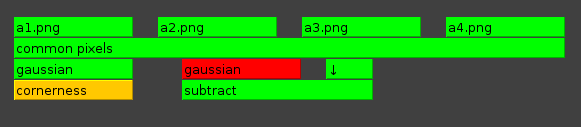
\includegraphics[width=\textwidth]{operatorstack.png}
\end{center}

The image pipeline is based on a directed acyclic graph. This graph represented
and is constructed from operators (\emph{nodes}) placed together in the \emph{operator
stack}. Each operator is represented by a box. Image data flows from top to
bottom. When two boxes touch vertically they are connected by an \emph{edge}.

So for example, in the image above, we have the following edges:
\begin{itemize}
\item $\texttt{a1.png} \rightarrow \texttt{common pixels}$
\item $\texttt{a2.png} \rightarrow \texttt{common pixels}$
\item $\texttt{a3.png} \rightarrow \texttt{common pixels}$
\item $\texttt{a4.png} \rightarrow \texttt{common pixels}$
\item $\texttt{common pixels} \rightarrow \texttt{gaussian}$
\item $\texttt{common pixels} \rightarrow \texttt{gaussian}$ (red)
\item $\texttt{common pixels} \rightarrow \texttt{$\downarrow$}$
\item $\texttt{gaussian}$ (red) $\rightarrow \texttt{subtract}$
\item $\texttt{$\downarrow$} \rightarrow \texttt{subtract}$
\item $\texttt{gaussian} \rightarrow \texttt{cornerness}$
\end{itemize}

(A \emph{passthrough} or \emph{identity} (do nothing) operator is represented by
a \texttt{$\downarrow$})

The reason this format is chosen instead of the traditional explicited edges is
simplicity and speed. The user no longer has to draw an edge between two nodes,
but can just place them on top of each other and achieve the same effect with
less screen clutter.

You can select an operator with the left or right mouse button. The \texttt{LMB}
does the primary (\emph{red}) selection. The output image of this operator is
then assigned to the upper \emph{image viewer}, the \emph{property panel} and
the \emph{histogram}.  The right mousebutton assigned a secondary selection
(orange), which is show in the lower image viewer and additionally can be show
as a overlay in the upper viewer (this can be useful to locate corner points, etc.).

Left or right clicking on the background deselects the operator.

\subsection{Image viewer}

\begin{center}
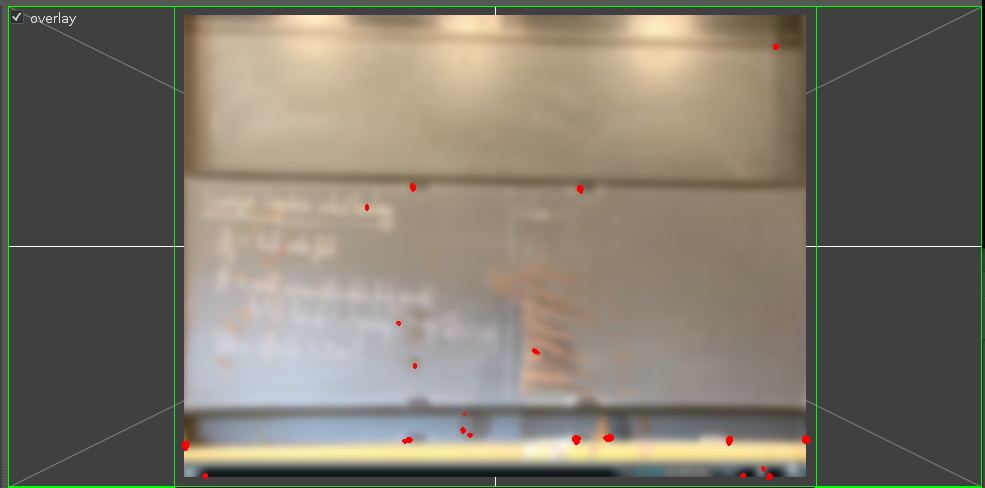
\includegraphics[width=\textwidth]{imageview.png}
\end{center}

The overlay checkbox in the top left corner is only visible when the lower
image is assigned (orange operator). For each pixel brighter than near black
a red circle is drawn in the upper image.

\subsection{Property Panel}

An operator can have some tweakable parameters, they are shown here as sliders.
The graph is not automatically recomputed at each change (only the current
operator) so one should click the \texttt{Compute} button in the top left
corner after modifying some parameters.

\begin{center}
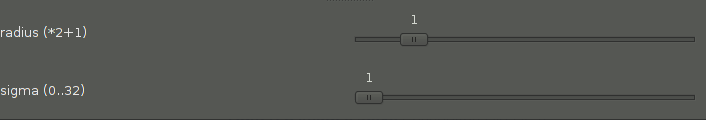
\includegraphics[width=\textwidth]{parameters.png}
\end{center}

\subsection{Histogram}
\begin{center}
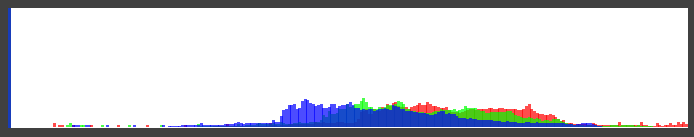
\includegraphics[width=\textwidth]{histogram.png}
\end{center}

The top left corner of the interface shows a histogram of the currently
selected operator (indicated in red in the operator stack).

\section{Implementation}
\subsection{Operators}
Operators can be implemented by extending the \texttt{Operator} class. The
following operators are implemented:
\begin{itemize}
\item Image arithmetic (for two images)
\item Cornerness measurement
\item Convolution with a kernel
\item The Euclidian norm of two images
\item Gaussian convolution
\item Grayscale conversion
\item Thresholding
\item Finding the \emph{odd-pixel-out} (explained below)
\end{itemize}

\subsection{Graph}
The operator stack is scanned and converted into an instance of \texttt{Graph}.
This graph then expresses the connections between operators. The operators are
computed in the order of a bread-first iteration of the graph. This makes sure
that depended operators are computed first.

Operators can support multiple distinct inputs, for instance for image
arithmetic and the odd-pixel-out operator.

\subsection{Properties}
A method in the operator class with an interger argument can be annotated using
\texttt{@Parameter}. Once an operator is selected it's methods are scanned and
parameter methods are bound to a slider in the property panel. This allows for
easy fine tuning.

\section{Erasing the lecturer}

The aim of the pipelines in this program is to take various pictures of a
person giving a lecture and removing the person from the lecture. The resulting
blackboard image should then be cropped at it's corners and the contents
converted to binary, the writing being one color and the board the other.

The pipelines themselves are fairly self explanatory; the operators in them
might need some explanation.

\subsection{Odd pixel out}
Let $p(x,y,t)$ represent our set of frames, where $(x,y)$ are obviously the
coordinates in the frame and $t$ is a time stamp (all integers). The input to
this operator should be three or more frames, ordered by increasing time stamp
$t$.

To erase the lecturer we asume he or she is moving around while the blackboard
is stable and writing is only \emph{added} to it.

The operator needs local pixel information only, thus, we can simplify to a
fixed $(x,y)$ position, so let $p_t=p(x,y,t)$ denote a single pixel at time
$t$.

So given a set of $p_0,\ldots,p_n$'s, we would like to figure out which color
occurs most frequently, because this would probably be the blackboard; the
second most frequent then is probably some chalk that was on frames $p_j$ for
$j > 2$ but not on $p_1$ and $p_2$. And so one.

What does this mean exactly? Well, ideally we would like to place the pixels in
bins corresponding to their colors $\pm \varepsilon$ for some $\varepsilon$ and
then sort the bins by number of items in it.
But we don't know beforehand how many bins, what $\varepsilon$ or what the mean
color of a subset of $p_i$'s we should pick. In fact, finding the optimum such
arrangement is a NP-hard problem. There are machine learning algorithms (for
instance \emph{$k$-means}) which can approximate this, but that seems a bit
heavy at this point. 

Another way to approach this problem is with an extra assumption: the teacher
is not overlapping in any of the frames. Then, given $p_1, p_2, p_3$ (say), we
want to find the pixel $p_l$ that is most different to all other pixels since
that would correspond the pixel of the moving lecturer. This distance can
computed by simply accumulating the distances to every other color and keeping
track of the pixel with the maximum such value. We discard this pixel and we
now have two pixels left. For the pixels in the output image we then take $p_i$
with maximum $i$, since the latest frame in this series contains the most
complete writing on the blackboard.

This is roughly how the odd-pixel operator works, see the \texttt{operators.CommonPixels}
class for details.

\subsection{Cornerness}

This is implemented as described in the lecture notes; but rather inefficiently
with several convolutions. Partial derivatives $\frac{\partial}{\partial x}$ and
$\frac{\partial}{\partial y}$ are approximated with a Sobel kernel.
The kernel can be scalar multiplied using a slider in the property panel.
For details, see the class \texttt{operators.Cornerness}.


\end{document}
